\documentclass[11pt,final]{amsart}

\usepackage{bm,url,xspace,verbatim}
\usepackage{amssymb,amsmath}
\usepackage[final,pdftex]{graphicx}
\usepackage[pdftex]{hyperref}


\newcommand{\ddt}[1]{\ensuremath{\frac{\partial #1}{\partial t}}}
\newcommand{\ddx}[1]{\ensuremath{\frac{\partial #1}{\partial x}}}
\newcommand{\ddy}[1]{\ensuremath{\frac{\partial #1}{\partial y}}}
\newcommand{\bU}{\mathbf{U}}
\newcommand{\eps}{\epsilon}
\newcommand{\grad}{\nabla}


\begin{document}

\title{Thoughts on marine ice sheets, motivated by MISMIP}
\author{Ed Bueler}
\date{\today}
\maketitle

I have been working on the PISM submission for MISMIP \cite{MISMIPwebpage}, and simultaneously reading \cite{SchoofMarine2} and \cite{SchoofMarine1}.  And it makes me think about marine ice sheets, continuity of flux, and (as usual) the quality of numerical solutions to PDEs.


\begin{figure}[ht]
%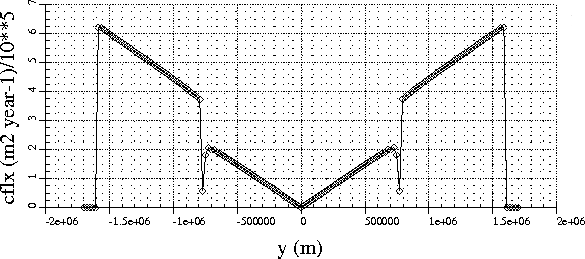
\includegraphics[width=4.5in,keepaspectratio=true]{cflxEBU1_1a_M1_A1}
%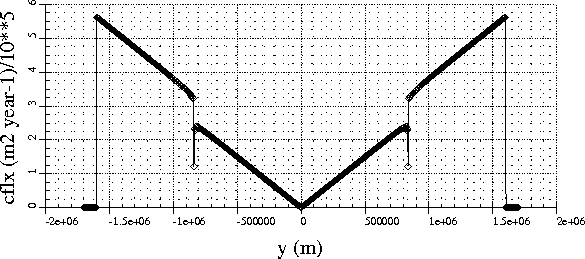
\includegraphics[width=4.5in,keepaspectratio=true]{cflxEBU1_1a_M3_A1}
A COUPLE OF OLD PISM RESULTS FROM MISMIP WENT HERE (FROM STABLE0.1)
\caption{Top: steady state ice flux $q=hu$, where $h$ is thickness and $u$ is horizontal velocity, for a MISMIP experiment using 150 grid spaces in the horizontal.  Bottom: the result when using four times grid refinement (600 spaces).}
\label{fig:badflux}
\end{figure}

PISM is not, for now, doing well on the continuity of flux at the grounding line.  In fact it is doing downright poorly, as shown in Figure \ref{fig:badflux}.\footnote{Figure \ref{fig:badflux} shows \texttt{EBU1\_1a\_M1\_A1} and \texttt{EBU1\_1a\_M3\_A1}.}  The figure should show straight lines on either side of the divide at $x=0$, instead of the jump and wiggle at the grounding line.  The flux jump \emph{is} of smaller magnitude when using the more refined grid, but it is still far too large.

PISM is apparently not doing well on getting the change of the steady position of the grounding line under parameter change, either.  (The softness parameter of ice $\bar A$ is the one changed in MISMIP.)

On the other hand, Christian is quite convincing in \cite{SchoofMarine2} that the boundary layer theory in \cite{SchoofMarine1} correctly predicts the position of the grounding line in this flow line case.  He is also convincing that numerical schemes can resolve their problems in the flow line case by sufficient grid refinement near the grounding line.  His numerical method does not model the ice shelf (not needed in the flow line case if the correct force is applied at the grounding line).  His scheme \emph{does} know the location of the grounding line, as he uses a stretched coordinate based the location of the grounding line.

These features of his numerical approach are each very hard to duplicate in the more realistic map-plane circumstances of a PISM Antarctica model, for instance.  It is desireable to avoid explicit parameterization of the grounding line as, for each model time, a curve in the map-plane.  It is not clear in several ways how to extend the boundary layer theory in \cite{SchoofMarine1} to the map-plane case.  Also the proposed grid refinement is much harder in the map-plane, both to implement a scheme and to make computation time scale well as the grid is refined.

In any case, the problem deserves consideration as a matter of pure numerical analysis.  That is, Christian and others have thought about what we should do to modify the obvious SSA equations to correctly account for physical effects.  But my approach is different: I am stuck with a numerical solver for the obvious SSA equations, but the solutions show badly behaved flux at steady state, so they are not getting solved well.  My question is, ``what about these obvious equations is causing the problem and how to fix it?''

My answer is this slogan:
\begin{quote}
\textbf{The main problem is that there is unbounded, singular function on the right side of the SSA force balance equation.  It is supposed to be there, but the numerical scheme can't handle it, in that the velocity gets a jump in it and then the coupled evolution of thickness and velocity exacerbates the jumps in velocity and flux.}
\end{quote}

To be clear on what I mean by the ``obvious SSA equations'', I will write the equations of the MISMIP ``category 2'' model, using the SSA \cite{WeisGreveHutter} on both sides of the grounding line and including an actual ice shelf model.  I'll stick to the flow line case here until I have made my point, which then applies to PISM's map plane case.  The ``obvious SSA equations'' are just two equations.  I'll write the equations and boundary conditions entirely in terms of two unknown functions, thickness $h(t,x)$ and horizontal velocity $u(t,x)$.  I'll freely adopt MISMIP notation and conventions, but we will need the HeavisidE function
	$$E(\xi) = \begin{cases} 0, & \xi<0, \\ 1, & \xi> 0 \end{cases}$$
in addition.

The two equations are, of course,
\begin{align}
&\ddt{h} + \ddx{}\left(h u\right) = a, \label{massconserveEARLY} \\
\ddx{}\Big[2 {\bar A}^{-1/n} h &\left|\ddx{u}\right|^{1/n-1} \ddx{u}\Big] - E(x_g-x) C|u|^{m-1} u = \text{RHS} \label{velocityEARLY}
\end{align}
where $a$ is the accumulation.  The boundary value problem is on the fixed interval $x\in[0,x_c]$, where $x=0$ is a divide and a location of symmetry, and $x=x_c$ is the calving front, which is kept at a fixed location.  The boundary condition at the calving front is given in the MISMIP description, and is not of greatest interest here.

The critical detail is what goes into the right hand side ``RHS'' of equation \eqref{velocityEARLY}.  Of course it is just the driving stress, and that seems simple, but I think it is not.  I found it helpful to at times forget what it means physically and concentrate on how regular/irregular it is.

One way to write the RHS is
\begin{equation}
\text{RHS} =  \rho_i g h \left[E(x_g-x) \ddx{(h-b)} + E(x-x_g) (1-\rho_i/\rho_w) \ddx{h}\right]. \label{RHSwxgONE}
\end{equation}
Note that the bed is at elevation $-b$ in the MISMIP language.  But the other way is
\begin{equation}
\text{RHS} =  ??????. \label{RHSwxgTWO}
\end{equation}

For the flow line case part of my point here is that there is just \emph{one} interval, from the divide all the way to the calving front, in a category 2 model.  We are solving a pair of equations with very irregular driving term, but it occurs in the middle of the interval $[0,x_c]$.  We don't need or want the explicit appearance of ``$x_g$'' in the equations.

In the map-plane case we can't even directly use Heaviside function notation this way.  To a mathematician I would say: ``in general the floating region is not a half-space or even a polygon.''

Let $\phi = \rho_w/\rho_i$ be the ratio of the density of sea water to that of ice.  Recall the floatation criterion
	$$\text{ice floats if } h < \phi b.$$
We can write the floatation criterion into the equations so that ``$x_g$'' will disappear:
\begin{align}
&\ddt{h} + \ddx{}\left(h u\right) = a, \label{massconserve} \\
\ddx{}\Big[2 {\bar A}^{-1/n} h &\left|\ddx{u}\right|^{1/n-1} \ddx{u}\Big] - E(h - \phi b) C|u|^{m-1} u = \text{RHS} \label{velocity}
\end{align}
where
	$$\text{RHS} = \rho_i g h \left[E(h - \phi b) \ddx{(h-b)} + E(\phi b - h) (1-\phi^{-1}) \ddx{h}\right].$$

I think this is useful conceptually because we see this pair of PDEs as ``autonomous'', i.e.~without explicit location dependence.  Certainly it generalizes to the map-plane case, where the corresponding right hand side\emph{s} have the vector formula

	\centerline{``$\text{RHS} = \rho_i g h \left[E(h - \phi b) \grad(h-b) + E(\phi b - h) (1-\phi^{-1}) \grad h\right]$.''}
\noindent Equations \eqref{massconserve} and \eqref{velocity} have well-known adaptations to two horizontal dimensions.

\bibliography{../../pism-dev/doc/ice_bib}
\bibliographystyle{siam}

\end{document}

